\section{Design and Modelling} \label{sec:design}
This section describes the design and architecture of the lab dashboard, highlighting how various components are implemented. It covers the data endpoint, defining what data enters the system and in what form, the mathematical models used to derive struggle and difficulty and the user interface design which exposes the analytics to educators. 
 
\subsection{System Architecture}

The proposed system adopts a layered architecture designed to support real-time learning analytics in computer lab environments. 
The architecture separates data generation, data ingestion and processing, as well as decision-making and action, into three distinct layers, ensuring each component can evolve independently. 

\begin{figure}[H]
    \centering
    \resizebox{\linewidth}{!}{%
    \begin{tikzpicture}[
        node distance = 0.9cm and 0.7cm,
        process/.style = {
            rectangle, draw, rounded corners=2pt,
            minimum width=2.7cm, minimum height=1.2cm,
            align=center, font=\small, fill=blue!4
        },
        store/.style = {
            rectangle, draw, rounded corners=2pt,
            minimum width=2.7cm, minimum height=1.2cm,
            align=center, font=\small, fill=gray!12
        },
        ui/.style = {
            rectangle, draw, rounded corners=2pt,
            minimum width=5.6cm, minimum height=1.4cm,
            align=center, font=\small, fill=violet!8
        },
        external/.style = {
            rectangle, draw, rounded corners=2pt,
            minimum width=2.7cm, minimum height=1.2cm,
            align=center, font=\small, fill=orange!12
        },
        flow/.style = {-{Stealth[length=2.4mm]}, thick},
        biflow/.style = {{Stealth[length=2.4mm]}-{Stealth[length=2.4mm]}, thick},
        grouplabel/.style = {font=\footnotesize\itshape, anchor=south, text=black!70},
        edgelabel/.style = {font=\scriptsize\itshape, fill=white, inner sep=1pt},
        layerlabel/.style = {font=\footnotesize\bfseries\itshape, anchor=east, text=black!60}
    ]
        % ===== Layer 1 - Data Generation =====
        \node[external] (students) {Students};
        \node[external, right=2.6cm of students] (endpoint) {AI Feedback\\Platform};
        \draw[flow] (students) -- node[edgelabel, above]{submissions} (endpoint);

        % ===== Layer 2 - Ingestion \& Processing =====
        \node[process, below=2.2cm of students] (ingest) {Data\\Ingestion};
        \node[store, right=of ingest] (caches) {Raw \&\\incorrectness\\caches};
        \node[process, right=of caches] (baseline) {Baseline\\Analytics};
        \node[process, right=of baseline] (advanced) {Advanced\\Models};
        \node[process, right=of advanced] (rag) {RAG\\Pipeline};

        % External LLM service, above the right end of the pipeline
        \node[external, above=1.3cm of rag] (llm) {LLM service\\(OpenAI)};

        % Dashed group around the swappable models cluster
        \begin{scope}[on background layer]
            \node[draw, dashed, rounded corners=3pt,
                  fit=(advanced),
                  inner sep=0.25cm] (modelgroup) {};
        \end{scope}
        \node[grouplabel] at (modelgroup.north) [yshift=2mm] {swappable subsystem};

        % Layer 2 internal flows
        \draw[flow] (endpoint.south) -- ++(0,-0.5) -| (ingest.north)
            node[edgelabel, pos=0.25, above]{poll};
        \draw[flow] (ingest) -- (caches);
        \draw[flow] (caches) -- (baseline);
        \draw[flow] (baseline) -- (advanced);
        \draw[flow] (advanced) -- (rag);
        \draw[flow] (baseline.north) to[bend left=35]
            node[edgelabel, pos=0.55]{incorrectness} (llm.west);
        \draw[flow] (rag.north) -- node[edgelabel, right]{generation} (llm.south);

        % ===== Layer 3 - Decision \& Action =====
        % Shared session state placed BETWEEN the two UIs so the file-locked
        % coordination between Instructor and Assistant is visually obvious.
        \node[ui, below=3.4cm of baseline, xshift=-5.2cm] (instructor)
            {Instructor Dashboard\\\footnotesize\itshape in-class, student detail, question detail};
        \node[store, right=0.5cm of instructor, minimum width=4.0cm, minimum height=1.4cm] (state)
            {Shared session state\\\footnotesize\itshape \texttt{lab\_session.json}\\(file-locked)};
        \node[ui, right=0.5cm of state] (assistant)
            {Lab Assistant Interface\\\footnotesize\itshape join, waiting, assigned};

        % Layer 2 -> Layer 3 flows (staggered bend depths per arrow to avoid shared horizontal channels)
        % Baseline -> Instructor (short L, near source)
        \draw[flow] (baseline.south) -- ++(0,-0.3) -|
            node[edgelabel, pos=0.25, above]{scores} (instructor.north);
        % Baseline -> Assistant (cross right, mid-depth bend)
        \draw[flow] (baseline.south) -- ++(0,-0.7) -| (assistant.north);

        % RAG -> Assistant (short L, near source)
        \draw[flow] (rag.south) -- ++(0,-0.3) -|
            node[edgelabel, pos=0.25, above]{feedback} (assistant.north);
        % RAG -> Instructor (cross far left, deepest bend)
        \draw[flow] (rag.south) -- ++(0,-1.0) -| (instructor.north);

        % Inter-UI coordination via file-locked shared session state (horizontal row)
        \draw[biflow] (instructor.east) -- (state.west);
        \draw[biflow] (state.east) -- (assistant.west);

        % Layer labels in the left margin
        \node[layerlabel] at ([xshift=-0.6cm]students.west) {Layer 1};
        \node[layerlabel] at ([xshift=-0.6cm]ingest.west) {Layer 2};
        \node[layerlabel] at ([xshift=-0.6cm]instructor.west) {Layer 3};
    \end{tikzpicture}}
    \caption{V2 system architecture: a three-layer pipeline from data ingestion through baseline and advanced analytics and the RAG pipeline to the instructor and lab-assistant surfaces, coordinated via the file-locked shared session state.}
    \label{fig: system architecture}
\end{figure}

\paragraph{Data Generation Layer}
As seen in Figure \ref{fig: system architecture}, student interactions form the primary source of data. When students submit an attempt or request feedback, the interaction data is recorded at the endpoint and not modified.

\paragraph{Data Ingestion and Processing Layer}
Data ingestion is performed periodically according to the user-defined refresh rate. Retrieved data will be stored in the raw data store, then parsed and normalised before being used for calculations. The data will be used to determine student struggle, question difficulty, and other required metrics.

\paragraph{Decision and Action Layer}
Data Analytics will now be sent to the learning dashboard for presentation to the instructor, thereby aiding decision-making. The instructor will identify students who are struggling. More complex questions will also be identified so that the instructor can go through the questions with the whole class. Instructors will use the dashboard to assign tasks to assistants to assist students who need help.

This layered design supports the project's aim of providing timely, targeted support during lab sessions while using the system as a decision-making tool for student support. Later sections build on this architecture.

\subsection{Data Endpoint} \label{sec: data endpoint}
A data endpoint is a specific URL or address in a web service or API that defines where and how clients can access the service. The proposed system integrates with the existing AI feedback platform through a single external data endpoint. The data endpoint is crucial in our system as it provides access to detailed records of student submissions and feedback interactions generated as students engage with lab questions. As outlined in Figure \ref{fig: system architecture}, the endpoint serves as the entry point to the analytics pipeline, supplying the raw data that will be processed, normalised, and aggregated for data visualisation. The integration is designed to be read-only, ensuring the data and metrics are not tampered with.

The endpoint returns an array in JSON format, where each record corresponds to a specific session based on the session's first submission time. Alongside standard fields such as module, question, timestamp and user, each record has an XML payload. The payload captures the interaction history for a given session, including submissions and AI responses. The design reflects the constraints of the existing system while providing vital information for our analytics.

Interaction data are organised around sessions, where a session represents a continuous period of student engagement from the first submission attempt. Within a session, students may have multiple submissions, getting multiple AI responses. This is beneficial in reflecting how their answers may improve question by question. The structure allows the capture of temporal patterns, repeated attempts, and help-seeking behaviour, which will be vital for identifying short-term struggle and difficult questions in lab sessions.

\begin{figure}[H]
    \centering
    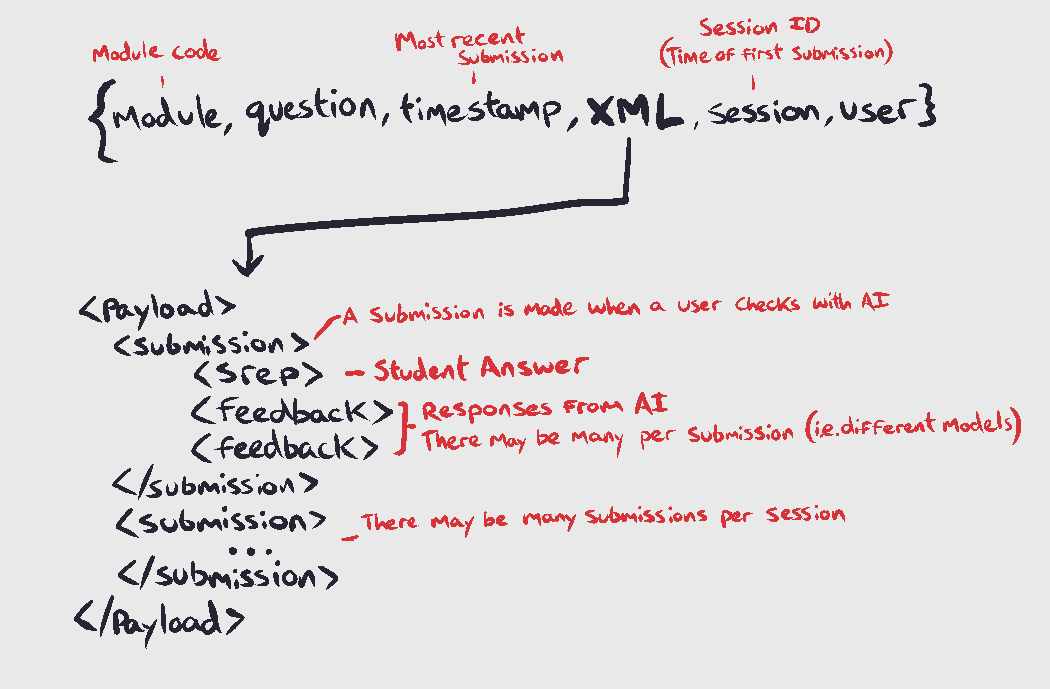
\includegraphics[width=1\linewidth]{figures/design-and-architecture/data-entry.png}
    \caption{Structure of session-based interaction data returned by feedback system}
    \label{fig: data entry}
\end{figure}

From the session-based data, the system derives a set of core metrics for real-time monitoring. These include attempts per question, time between attempts, AI-based indicators of correctness, and the frequency with which students request feedback. By using these, we will enable the system to distinguish among students and identify those who are struggling the most. The derived metrics will form the basis of our two key metrics: student struggle and question difficulty.

It is essential to consider that we may receive incomplete or noisy data during sessions, which could stem from students repeatedly returning to the AI feedback system or from procrastination on their work. Not all indicators of struggle and question difficulty are valuable on their own; hence, they are combined to produce indicators of student struggle and question difficulty.



\subsection{Baseline Analytics Design}
This section describes the baseline metrics, student struggle and question difficulty and the data from the endpoint that is used to derive them.
\subsubsection{Student Struggle Model} \label{sec: student struggle}

\paragraph{Modelling Objective}
To model student struggle, let $s$ denote a student and $\sigma$ denote the session. We will denote students who struggle with a scalar function:
\begin{equation}
    S(s,\sigma) \in [0,1]
\end{equation} \label{eq: scalar in range model}
The student struggle function will allow us to quantify the degree of difficulty that students $s$ are currently experiencing during session $\sigma$, based on the observable data from the endpoint in Section \ref{sec: data endpoint}. The model will support real-time prioritisation in computer labs.

\paragraph{Identified Variables}
From the session-based interaction data described in Section \ref{sec: data endpoint}. We can derive the following quantities:
\begin{itemize}
    \item $n_{s,\sigma}$ - The total number of submissions made by a student $s$ during session $\sigma$
    \item $t_{s,\sigma}$ - The total active time elapsed during session $\sigma$
    \item $i_{s,\sigma}$ - The average AI incorrectness measure for student $s$ during session $\sigma$, derived from AI-Based answer ratings
    \item $r_{s,\sigma}$ - The number of retry submissions within session $\sigma$
    \item $d_{s,\sigma}$ - The regression slope of incorrectness scores against the submission index, which captures whether a student is improving or deteriorating across the session
    \item $\mathrm{rep}_{s,\sigma}$ - The number of exact-match repeated submissions within session $\sigma$
\end{itemize}
By leveraging metrics linked to student struggle, we can produce a student struggle score

\paragraph{AI-Based Answer Rating}
Let $A_{s,\sigma,k}$ be the $k$-th submitted answer by student $s$ in session $\sigma$. We will derive an LLM-based scoring function. Where $Q_{\sigma}$ is the current question and $A_{\sigma}$ is the answer, we will define our LLM-based scoring function to be:
\begin{equation}
    c_{s,\sigma,k} = C(A_{s,\sigma,k},A_{\sigma},Q_{\sigma}) \in [0,1]
\end{equation}
where $c_{s,\sigma,k}$ is the correctness measure that measures the quality of a students answer, where 1 is the correct answer and 0 is completely wrong. We can then define our incorrectness measure:
\begin{equation}
    i_{s,\sigma,k} = 1 - c_{s,\sigma,k} \in [0,1]
\end{equation}

\paragraph{Normalisation}

The retry rate, repetition rate and trajectory slope are derived from the counts identified earlier:

\begin{equation*}
    \tilde{r}_{s,\sigma} = \frac{r_{s,\sigma}}{n_{s,\sigma}} \in [0,1], \qquad
    \tilde{\mathrm{rep}}_{s,\sigma} = \frac{\mathrm{rep}_{s,\sigma}}{n_{s,\sigma}} \in [0,1].
\end{equation*}

The trajectory slope $d_{s,\sigma}$ is signed (negative values indicate improvement, positive values indicate deterioration) and therefore unbounded by definition. The mean incorrectness $i_{s,\sigma}$ and the time decayed recent-incorrectness $A^{raw}(s,\sigma)$ are already bounded to $[0,1]$ by construction as each is an average of values already in $[0,1]$.

To ensure each component contributes the weighting intended, every signal is min-max normalised across the cohort for the session with:
\begin{equation*}
    \hat{x}_{s,\sigma}
    = \frac{x_{s,\sigma} - x_{\min}}{x_{\max} - x_{\min}},
    \qquad
    x_{\min} = \min_{s' \in S} x_{s',\sigma}, \quad
    x_{\max} = \max_{s' \in S} x_{s',\sigma}.
\end{equation*}
Applied to the seven signals introduced earlier, we have:
\begin{equation*}
    \hat{n}_{s,\sigma},\;
    \hat{t}_{s,\sigma},\;
    \hat{\imath}_{s,\sigma},\;
    \hat{\tilde{r}}_{s,\sigma},\;
    \widehat{A^{\mathrm{raw}}}(s,\sigma),\;
    \hat{d}_{s,\sigma},\;
    \widehat{\tilde{\mathrm{rep}}}_{s,\sigma}
    \;\in\; [0,1].
\end{equation*}
Min-max normalisation is applied even to signals already bounded to $[0,1]$, because the configured weights only match the effective contribution of each signal when every signal occupies the full $[0,1]$ range, otherwise a signal that clusters in a sub-interval would contribute less than the weight implied. 
When $x_{\min} = x_{\max}$, the normalised value is conventionally set to $0$.


\paragraph{Recent submissions weighted by time decay}
To reflect that recent submissions are more indicative of current struggle than older submissions in a live setting, each submission is weighted by an exponential decay in the time elapsed since it was made, rather than its position in its submission sequence. 
Let $\Delta_{s,\sigma,k}$ denote the elapsed time in seconds between submission $k$ and the current refresh. The time-decay weight is defined as:
\begin{equation}
    w_{s,\sigma,k} = \exp\!\left(-\frac{\ln 2}{H}\,\Delta_{s,\sigma,k}\right),
    \label{eq:time-decay-weight}
\end{equation}
where $H = 1800$ s is the half-life; a submission made 30 minutes ago contributes half the weight of a submission made just now. 
The recent-incorrectness signal is then the time-decay weighted mean of the per-submission incorrectness:

\begin{equation}
    A^{\mathrm{raw}}(s,\sigma)
    = \frac{\sum_{k=1}^{n_{s,\sigma}} w_{s,\sigma,k}\, i_{s,\sigma,k}}
           {\sum_{k=1}^{n_{s,\sigma}} w_{s,\sigma,k}}
    \;\in\; [0,1].
    \label{eq:a-raw}
\end{equation}
Time-based decay is preferred over position-based weighting because students submit at irregular intervals. Weighting by elapsed time gives a more accurate reflection of current struggle rather than submission position. 
Since each $i_{s,\sigma,k} \in [0,1]$, and the weights are positive, the convex combination $A^{\mathrm{raw}}(s,\sigma)$ is bounded in $[0,1]$ by construction, and does not require normalisation.
    
\paragraph{Struggle Score Definition}
The raw student struggle is a convex combination of the seven bounded components:
\begin{equation}
    \label{eq:struggle-raw}
    S^{\mathrm{raw}}(s,\sigma)
    = \alpha \hat{n}_{s,\sigma}
    + \beta  \hat{t}_{s,\sigma}
    + \gamma \hat{\imath}_{s,\sigma}
    + \delta \hat{\tilde{r}}_{s,\sigma}
    + \eta   \widehat{A^{\mathrm{raw}}}(s,\sigma)
    + \zeta  \hat{d}_{s,\sigma}
    + \theta \widehat{\tilde{\mathrm{rep}}}_{s,\sigma},
\end{equation}
where the coefficients are non-negative and sum to one:
\begin{equation*}
    \alpha,\beta,\gamma,\delta,\eta,\zeta,\theta \geqslant 0,
    \qquad
    \alpha+\beta+\gamma+\delta+\eta+\zeta+\theta = 1.
\end{equation*}
The default values used in the deployed system are:
\begin{equation*}
    \alpha = 0.10, \quad
    \beta = 0.10, \quad
    \gamma = 0.20, \quad
    \delta = 0.10, \quad
    \eta = 0.38, \quad
    \zeta = 0.05, \quad
    \theta = 0.07,
\end{equation*}
summarised by signal in Table \ref{tab: struggle weights}. The recent-incorrectness signal carries the largest weight ($\eta = 0.38$) because the model prioritises within-session struggle over cumulative behaviour. 
The longer tail signals (trajectory and repetition) carry small but non-zero weights so they can break ties between students who look similar on the headline metrics. 
The weights were tuned by trial and error in the absence of labelled ground-truth data. 
Since every component is bounded in $[0,1]$ and all the weights are convex,
\begin{equation*}
    S^{\mathrm{raw}}(s,\sigma) \in [0,1].
\end{equation*}

The weights set above are the baseline model (v1) and remain the system default.
As an alternative weighting approach, we obtained second-opinion labels from an LLM rater and re-fitted both the struggle model of Table~\ref{tab: struggle weights} and the difficulty model of Table~\ref{tab: difficulty weights} as a v2 model variant.
The trained model can be toggled on at runtime in the V2 React dashboard from the Settings view.
The v2 model vectors are signed and do not satisfy the convex combination constraint of Equation~\ref{eq: scalar in range model} which is a consequence of using ordinary least-squares linear regression for fitting; the v1 model is preserved as the deployed default for the system. The pipeline that produced the v2 vectors is described in Section~\ref{sec:v2-pipeline-design}; the model comparison is reported in Section~\ref{sec:eval-results}.

\begin{table}[H]
    \centering
    \begin{tabular}{|p{0.15\textwidth}|p{0.55\textwidth}|p{0.20\textwidth}|}
    \hline
    \textbf{Symbol} & \textbf{Meaning} & \textbf{Weight} \\
    \hline
    $\hat{n}_{s,\sigma}$ & Submission count (min-max normalised) & $\alpha = 0.10$ \\
    \hline
    $\hat{t}_{s,\sigma}$ & Active time (min-max normalised) & $\beta = 0.10$ \\
    \hline
    $\hat{\imath}_{s,\sigma}$ & Mean LLM incorrectness (min-max normalised) & $\gamma = 0.20$ \\
    \hline
    $\hat{\tilde{r}}_{s,\sigma}$ & Retry rate (min-max normalised) & $\delta = 0.10$ \\
    \hline
    $\widehat{A^{\mathrm{raw}}}(s,\sigma)$ & Time-decayed recent incorrectness (min-max normalised) & $\eta = 0.38$ \\
    \hline
    $\hat{d}_{s,\sigma}$ & Improvement-trajectory slope (min-max normalised) & $\zeta = 0.05$ \\
    \hline
    $\widehat{\tilde{\mathrm{rep}}}_{s,\sigma}$ & Answer-repetition rate (min-max normalised) & $\theta = 0.07$ \\
    \hline
    \end{tabular}
    \caption{Seven signals contributing to the baseline student struggle score $S^{\mathrm{raw}}(s,\sigma)$, with default weights; weights sum to $1.00$}
    \label{tab: struggle weights}
\end{table}

\paragraph{Bayesian shrinkage towards the class mean}
A student with very few submissions can produce a $S^{\mathrm{raw}}$ that is dominated by noise; a student with two submissions may register a $100\%$ retry rate purely because the second submission was a repeat of a question, without that being indicative of struggle. 
To stabilise scores when the per-student observation count is small, $S^{\mathrm{raw}}$ is shrunk toward the class mean with a weight that depends on the student's submission count $n_{s,\sigma}$:
\begin{equation}
    S^{\mathrm{shrunk}}(s,\sigma)
    = \frac{n_{s,\sigma}}{n_{s,\sigma} + K}\,S^{\mathrm{raw}}(s,\sigma)
    + \frac{K}{n_{s,\sigma} + K}\,\bar{S}^{\mathrm{raw}}_{\sigma},
    \label{eq:struggle-shrunk}
\end{equation}
where $\bar{S}^{\mathrm{raw}}_{\sigma}$ is the cohort mean of the raw struggle in session $\sigma$ and $K$ is a hyper-parameter controlling the strength of the shrinkage. The default value is $K=5$, so a student with $n_{s,\sigma} \gg 5$ submissions is essentially unaffected while a student with $n_{s,\sigma} \ll 5$ submissions is shrunk close to the class mean. 
The technique is the classical empirical Bayes shrinkage estimator in the tradition of James-Stein and Efron \& Morris \cite{efronSteinsParadoxStatistics1977}, here in the conjugate-prior form in which $K$ acts as a prior count \cite{morrisParametricEmpiricalBayes1983}. It is applied here at the level of the aggregate struggle score rather than at the level of the individual signals. 
Shrinkage and temporal smoothing serve complementary roles, where shrinkage handles cold-start uncertainty and temporal smoothing handles noise when refreshing scores within a session.

\paragraph{Temporal updating for real-time operation}
To provide a responsive, stable indicator, we will update struggle with exponential smoothing:
\begin{equation}
    S_t(s,\sigma) = (1-\lambda)S_{t-1}(s,\sigma) + \lambda S^{\mathrm{shrunk}}(s,\sigma), \quad \lambda \in (0,1]
    \label{eq: temporal struggle}
\end{equation} 
It follows that the update preserves boundaries, giving:
\begin{equation*}
    S_t(s,\sigma) \in [0,1], \quad  \forall t
\end{equation*}

\paragraph{Interpretation of model}
Higher values of $S_t(s,\sigma)$ indicate that student $s$ is experiencing sustained difficulty in the current session. The metric in Equation \ref{eq: temporal struggle} will prove to be valuable in real-time prioritisation of help in lab sessions. This measure does not indicate student ability in the cohort but rather in lab struggle.

\subsubsection{Temporal Smoothing}
Live struggle scores carry noise from two sources. Within a single score computation, submissions arrive at irregular intervals, so recent submissions should count more than older ones. Across refresh cycles, a student's score can change even when nothing meaningful has happened.
Both techniques were introduced in the previous section; this subsection names them explicitly and contrasts their roles.

\paragraph{Per-submission time decay inside $A^{\mathrm{raw}}$}

The first mechanism reweights submissions within a single computation of $S^{\mathrm{raw}}$.
Each submission contributes to the recent-incorrectness signal $A^{\mathrm{raw}}(s,\sigma)$ with a weight that decays exponentially with the time elapsed since the submission was made, as defined in Equations~\ref{eq:time-decay-weight} and~\ref{eq:a-raw}. 
The half-life is fixed at $H = 1800$ s, so a submission made 30 minutes ago contributes half the weight of a submission made just now. 
Because students submit at irregular intervals, time-based decay gives a more accurate reflection of current struggle than index-based weighting.

\paragraph{Exponentially Weighted Moving Average (EWMA) across refresh cycles applied to $S^{\mathrm{shrunk}}$}

The second mechanism stabilises the score in between refresh cycles. 
After the raw struggle score is computed and shrunk toward the cohort mean (Equation~\ref{eq:struggle-shrunk}), the resulting $S^{\mathrm{shrunk}}$ is smoothed across refresh cycles using a standard exponentially weighted moving average (EWMA), as given by Equation~\ref{eq: temporal struggle}.

The smoothing rate $\lambda = 0.3$ is fixed by the configuration constant \texttt{SMOOTHING\_ALPHA}, gated on by \texttt{SMOOTHING\_ENABLED} (which will be left active by default but can be toggled off). 
A small $\lambda$ trusts past observations more, giving a smoother trajectory, while a larger $\lambda$ trusts the current shrunk score more, giving a more responsive trajectory. 
The chosen value of $\lambda = 0.3$ was tuned by trial and error to give a good balance between responsiveness and stability, in the absence of labelled ground-truth data. 

\begin{table}[H]
    \centering
    \begin{tabular}{|p{0.22\textwidth}|p{0.34\textwidth}|p{0.34\textwidth}|}
    \hline
    \textbf{Property} & \textbf{Per-submission decay} & \textbf{EWMA across refresh} \\
    \hline
    What it smooths & Submissions inside one $A^{\mathrm{raw}}$ computation & The final score $S$ across refresh cycles \\
    \hline
    Granularity & Per submission (seconds) & Per refresh tick (typically every few seconds) \\
    \hline
    Decay parameter & Half-life $H = 1800$ s & Smoothing rate $\lambda = 0.3$ \\
    \hline
    Recurrence form & Weight $\exp(-\ln 2 / H \cdot \Delta)$ on each submission & $S_t = (1-\lambda)S_{t-1} + \lambda S^{\mathrm{shrunk}}$ \\
    \hline
    Noise it suppresses & Old submissions dominating a still-active student & Score fluctuations across refresh ticks \\
    \hline
    Source of the problem & Irregular submission intervals within one session & Single-submission fluctuations between refreshes \\
    \hline
    \end{tabular}
    \caption{The two temporal-smoothing mechanisms in the baseline struggle model and the role each plays.}
    \label{tab: temporal smoothing}
\end{table}

\subsubsection{Question Difficulty Model} \label{sec: task difficulty}

\paragraph{Modelling Objective}
To model question difficulty, let $q$ denote a question during the lab session, and let $\mathcal{S}_q$ denote the set of student-session pairs associates with task q. We will denote questions that are difficult with a scalar function:
\begin{equation}
    D(q) \in [0,1]
\end{equation}
The question difficulty function will allow us to quantify the degree of difficulty of a question $q$, that the students in the $\mathcal{S}_q$ set are finding the hardest, based on the observable data from the endpoint in Section \ref{sec: data endpoint}. The model will support real-time prioritisation in computer labs

\paragraph{Identified Variables}
From the session based interaction data described in Section \ref{sec: data endpoint}, the following quantities are derived. 
A submission is treated as correct if its LLM-derived incorrectness score $i_{s,\sigma,k}$ is below a fixed threshold of $\tau$. 
The system uses $\tau = 0.5$ by default.
\begin{itemize}
    \item $n_{q}$ - The total number of attempts on question $q$
    \item $c_{q}$ - The total number of correct attempts on question $q$
    \item $t_{q}$ - The average time spent on question $q$
    \item $a_{q}$ - The average number of attempts spent on question $q$
    \item $f_{q}$ - Average AI incorrectness measure for $q$, derived from AI-Based answer ratings
    \item $p_{q}$ - The number of students whose first attempt at $q$ was incorrect
\end{itemize}
By leveraging metrics linked to question difficulty, we can produce a question difficulty score.

\paragraph{Normalisation}
The incorrect rate and first-attempt failure rate are derived from the counts identified above: 
\begin{equation*}
    \tilde{c}_{q} = 1 - \frac{c_{q}}{n_{q}} \in [0,1], 
    \qquad
    \tilde{p}_{q} = \frac{p_{q}}{|\mathcal{S}_{q}|} \in [0,1],
\end{equation*}
The average time and average attempts are min-max normalised across the cohort of questions in the current session:
\begin{equation*}
    \tilde{t}_{q} = \frac{t_{q} - t_{\min}}{t_{\max} - t_{\min}} \in [0,1],
    \qquad
    \tilde{a}_{q} = \frac{a_{q} - a_{\min}}{a_{\max} - a_{\min}} \in [0,1].
\end{equation*}
The average LLM incorrectness $f_{q}$ is already bounded by construction, so:
\begin{equation*}
    \tilde{f}_{q} = f_{q} \in [0,1].
\end{equation*}



\paragraph{Difficult Task Definition}
Question difficulty is defined as a convex combination of the five bounded components:
\begin{equation}
    D^{\mathrm{raw}}(q)
    = \alpha\,\tilde{c}_{q}
    + \beta\,\tilde{t}_{q}
    + \gamma\,\tilde{a}_{q}
    + \delta\,\tilde{f}_{q}
    + \epsilon\,\tilde{p}_{q},
    \label{eq:difficulty-raw}
\end{equation}
where the coefficients are non-negative and sum to one:
\begin{equation*}
    \alpha,\beta,\gamma,\delta,\epsilon \geqslant 0,
    \qquad
    \alpha+\beta+\gamma+\delta+\epsilon = 1.
\end{equation*}
The default values used in the deployed system are:
\begin{equation*}
    \alpha = 0.28, \quad
    \beta  = 0.12, \quad
    \gamma = 0.20, \quad
    \delta = 0.20, \quad
    \epsilon = 0.20,
\end{equation*}
summarised by signal in Table \ref{tab: difficulty weights}.  Since every component is bounded in $[0,1]$ and the combination is convex:
\begin{equation*}
    D^{\mathrm{raw}}(q) \in [0,1].
\end{equation*}

\begin{table}[H]
    \centering
    \begin{tabular}{|p{0.15\textwidth}|p{0.55\textwidth}|p{0.20\textwidth}|}
    \hline
    \textbf{Symbol} & \textbf{Meaning} & \textbf{Weight} \\
    \hline
    $\tilde{c}_{q}$ & Incorrect rate, $1 - c_q/n_q$ & $\alpha = 0.28$ \\
    \hline
    $\tilde{t}_{q}$ & Average time per student (min-max normalised) & $\beta = 0.12$ \\
    \hline
    $\tilde{a}_{q}$ & Average attempts per student (min-max normalised) & $\gamma = 0.20$ \\
    \hline
    $\tilde{f}_{q}$ & Average LLM incorrectness score & $\delta = 0.20$ \\
    \hline
    $\tilde{p}_{q}$ & First-attempt failure rate, $p_q/|\mathcal{S}_q|$ & $\epsilon = 0.20$ \\
    \hline
    \end{tabular}
    \caption{Five signals contributing to the baseline question difficulty score $D^{\mathrm{raw}}(q)$, with default weights; weights sum to $1.00$.}
    \label{tab: difficulty weights}
\end{table}


\paragraph{Temporal updating for real-time operation}
To provide a responsive stable indicator, we will update question difficulty with exponential smoothing across refresh cycles:
\begin{equation}
    D_t(q) = (1-\lambda)\,D_{t-1}(q) + \lambda\,D^{\mathrm{raw}}(q), \quad \lambda \in (0,1].
    \label{eq: temporal difficulty}
\end{equation}

\paragraph{Interpretation of Model}
Higher values of $D_t(q)$ indicate that a question is difficult for the class as a whole during the current session. The metric will prove to be valuable in real-time prioritisation of help in lab sessions.

\subsubsection{Alternative Modelling Approach: Collaborative Filtering}

\paragraph{Motivation}
The parameter-based struggle model defined in Section \ref{sec: student struggle} assigns a score to each student independently base on a weighted combination of normalised interaction features. Whilst this approach is computationally lightweight and interpretable, it depends on the weightings  $\alpha, \beta, \gamma, \delta, \eta$. We can use an alternative modelling approach based on Collaborative Filtering, where rather than scoring each student in isolation, we explore similarity between students.

\paragraph{Student Interaction Matrix}

Let $\mathcal{S} = \{s_1,s_2,\ldots, s_n\}$ denotes the set of students present in sessions $\sigma$. For each student $s_i$, we define a five-dimensional feature vector derived from the normalised interaction quantities introduced in Section \ref{sec: student struggle}:

\begin{equation}
    \mathbf{x}_{s_i} =
    \begin{pmatrix}
        \hat{n}_{s_i,\sigma},\;
        \hat{t}_{s_i,\sigma},\;
        \hat{\imath}_{s_i,\sigma},\;
        \widehat{A^{\mathrm{raw}}}(s_i, \sigma),\;
        \hat{d}_{s_i,\sigma}
    \end{pmatrix}^{\top}
    \in [0,1]^5
\end{equation}

Collecting these vectors row-wise, we define the student interaction matrix:

\begin{equation}
    \mathbf{X} \in [0,1]^{n \times 5}, \quad \mathbf{X}_{ij} = [\mathbf{x}_{s_i}]_j
\end{equation}

Each row of $\mathbf{X}$ encodes one student's current behavioural profile during the session. The matrix is updated at each refresh interval as new data arrives from the endpoint.

\paragraph{Student Similarity Measure}
To quantify how similar two students are, we apply cosine similarity over their feature vectors. Cosine similarity is preferred over Euclidean distance because it measures the angle between two vectors rather than their absolute magnitudes, making it robust to differences in overall activity levels between students.

\begin{equation}
    \text{sim}(s_i, s_j) =
    \frac{\mathbf{x}_{s_i}^{\top} \mathbf{x}_{s_j}}
         {\|\mathbf{x}_{s_i}\|_2 \cdot \|\mathbf{x}_{s_j}\|_2}
    \in [0, 1]
\end{equation}

Since all components of $\mathbf{x}_{s_i}$ are normalised to $[0,1]$, the dot product is non-negative, and cosine similarity is bounded to $[0,1]$. This yields a symmetric similarity matrix
$\mathbf{W} \in [0,1]^{n \times x}$ where $W_{ij} = \text{sim}(s_i,s_j)$ and $W_{ii} = 1$ by definition. A value close to 1 indicates near identical behavioural profiles, whilst a value close to 0 indicates students with very different profiles.

\paragraph{Help-Seeking as a Proxy for Struggle}
In traditional systems, user ratings serve as the signal across similar users. In the lab setting, no explicit ratings are available, so we define a binary help seeking indicator derived from the parametrix model as a proxy:

\begin{equation}
    h_{s,\sigma} =
    \begin{cases}
        1 & \text{if } S_t(s,\sigma) \geq \tau \\
        0 & \text{otherwise}
    \end{cases}
\end{equation}

where $\tau \in {0,1}$ is a threshold above which a student is considered to be observably struggling based on their score. This allows collaborative filtering to leverage signals from students who are struggling with similar peers who may not have crossed the threshold, enabling earlier intervention.

\paragraph{Predicted Help Need with $k$-Nearest Neighbours}
For a student $s$ for whom $h_{s,\sigma}$, we estimate their latent help need by aggregating the help-seeking behaviour of their $k$ most similar peers.
Let $\mathcal{N}_k(s)$ denotes the set of $k$ students with the highest similarity to $s$, excluding $s$:

\begin{equation}
    \mathcal{N}_k(s) = \underset{
        s' \in \mathcal{S} \setminus \{s\},\; |\mathcal{N}| = k
    }{\arg\text{top-}k}\; \text{sim}(s, s')
\end{equation}

The predicted help-need score is then defined as a similarity-weighted average of the help indicators of the $k$ nearest neighbours.


\begin{equation}
    \hat{h}_{s,\sigma} =
    \frac{\displaystyle\sum_{s' \in \mathcal{N}_k(s)} \text{sim}(s, s') \cdot h_{s',\sigma}}
         {\displaystyle\sum_{s' \in \mathcal{N}_k(s)} \text{sim}(s, s')}
    \in [0, 1]
\end{equation}

A high value of $\hat{h}_{s,\sigma}$ indicates that student $s$ is similar to peers who required help, suggesting they may benefit from intervention.

\paragraph{Comparison with Parameter-Based Model}
Table~\ref{tab: model comparison} summarises the key structural differences 
between the adopted parametric model and the collaborative filtering 
alternatively, highlighting the properties that informed the choice of 
primary approach.

\begin{table}[H]
    \centering
    \begin{tabular}{|p{0.25\textwidth}|p{0.33\textwidth}|p{0.33\textwidth}|}
    \hline
    \textbf{Property} & \textbf{Parameter-Based Model} & \textbf{Collaborative Filtering} \\
    \hline
    Scoring basis & Weighted formula & Peer similarity \\
    \hline
    Interpretability & High & Moderate \\
    \hline
    Cold start & Immediate & Requires $\geq k+1$ active students \\

    \hline
    Computational complexity & $O(n)$ per update & $O(n^2)$ per update \\
    \hline
    \end{tabular}
    \caption{Structural comparison of the parametric struggle model and the 
    collaborative filtering alternative}
    \label{tab: model comparison}
\end{table}

\paragraph{Justification for Current Approach}
The parameter-based model is adopted as the primary approach for several reasons. This approach does not require a minimum class size to be considered viable, making it robust to sessions with few students where the similarity matrix $\mathbf{W}$ would be unreliable. Additionally, it produces more reliable results immediately, whereas a collaborative filtering approach produces results that are not reliable at the start of a session. 

The collaborative filtering approach is implemented alongside the parameter-based model as a secondary indicator, exposed through the Settings panel as a user-toggle option like Bloomberg's terminal; it is enabled by default with $k=3$ nearest neighbours and a configurable elevation threshold, and can be turned off if the instructor prefers the parametric model.

\subsubsection{Mistake Clustering} \label{sec: mistake clustering}

Beyond aggregate difficulty, instructors benefit from seeing what kind of mistakes students are making on a given question. 
The system clusters incorrect submissions per question so that dominant error patterns are surfaced rather than left hidden behind a single “incorrect” count. 
The pipeline combines three standard text-mining techniques - TF-IDF vectorisation, $k$-means clustering, and silhouette-based model selection - followed by an LLM labelling step that attaches human-readable descriptions to the clusters. The formal definitions of TF-IDF \cite{saltonVectorSpaceModel1975,manningIntroductionInformationRetrieval2006}, $k$-means \cite{MacQueen1967SomeMF,arthurKmeansAdvantagesCareful}, and the silhouette coefficient \cite{rousseeuwSilhouettesGraphicalAid1987} are described in Section~\ref{sec: text mining}; this section describes the design choices specific to the lab setting.

\paragraph{Pipeline} 
For each question $q$, the incorrect submissions (those whose LLM-derived incorrectness score $i_{s,\sigma,k}$ is above the threshold $\tau$) are vectorised using TF-IDF over their answer text. 
$k$-means clustering is then applied for each $k$ in a small range, and the value that maximises the mean silhouette coefficient is selected automatically, removing the need for the instructor to specify a target cluster count.  
\begin{equation}
    k^\star = \arg\max_{k \in \{2,\ldots,K_{\max}\}} \frac{1}{|X_q|} \sum_{x \in X_q} s(x; k),
    \label{eq:cluster-auto-k}
\end{equation}
Once clusters are formed, a generative model is prompted with a sample of representative answers from each cluster to produce a short natural language label \cite{wangGoalDrivenExplainableClustering2023}, which is displayed alongside the cluster in the Question Detail View. 

\paragraph{Parameters and Gating}
Clustering is only attempted when at least $N_{\min} = 3$ incorrect submissions are available for question $q$; below this threshold the noise in cluster assignments outweighs any pattern they might reveal, and the question is shown without clusters. 
The silhouette sweep evaluates $k \in \{2, \ldots, K_{\max}\}$ with $K_{\max} = 5$; mistake patterns within a single lab question rarely partition into more than five qualitatively distinct groups. 
For each surfaced cluster, up to three representative answers are shown in the UI so the instructor can verify the cluster's coherence at a glance.

\paragraph{Interpretation}
Where the question difficulty score $D_t(q)$ indicates whether a question is causing trouble, the mistake clustering provides insight into what kind of trouble it is causing. 
This complements the parametric difficulty signal: a question may register as "Medium" overall but reveal a single dominant error pattern affecting most struggling students, in which case the appropriate intervention is to address that misconception with a class-wide explanation rather than helping students one-on-one.

\subsection{Advanced Model Design}

\subsubsection{Measurement Confidence} \label{sec: measurement confidence}

Every incorrectness score $i_{s,\sigma,k}$ in this design is derived from an LLM judgement that is uncertain. To prevent the instructor from over-interpreting unreliable scores, each submission also carries a confidence measurement value $\kappa_{s,\sigma,k} \in [0,1]$ that quantifies how trustworthy the corresponding incorrectness estimate is, in the spirit of classical test theory \cite{lord1968statistical}.

The confidence is composed of two factors and a base multiplier:
\begin{equation}
    \kappa_{s,\sigma,k}
    = \kappa_0 \cdot \mathrm{length}(A_{s,\sigma,k}) \cdot \Big(\tfrac{1}{2} + \tfrac{1}{2}\,\mathrm{extremity}(i_{s,\sigma,k})\Big),
    \label{eq:measurement-confidence}
\end{equation}
where $\kappa_0 \in [0,1]$ is a base confidence value and each of the two factors is bounded in $[0,1]$. The $\mathrm{length}$ factor penalises very short submissions for which the model has little signal to work with; the $\mathrm{extremity}$ factor rewards scores near the endpoints $0$ and $1$ over middling values, reflecting that the model is most certain when an answer is clearly correct or wrong and least certain when an answer is borderline. Submissions with empty or missing feedback are assigned $\kappa = 0$. The half-and-half scaling on the extremity term ensures that valid submissions with mid-range scores still receive at least half of the base confidence, prioritising smooth degradation over hard cut-offs.


In the dashboard, $\kappa$ is surfaced as a coloured indicator next to the incorrectness value in the Question Detail view: green when $\kappa$ exceeds a high threshold (trust the score), amber for intermediate values (verify before acting), and grey when $\kappa$ falls below a low threshold (the score should not drive intervention decisions on its own). This makes the uncertainty visible to the instructor without requiring them to read the underlying score.


\subsubsection{Item Response Theory}  \label{sec: irt}
The baseline difficulty score $D_t(q)$ defined in Section \ref{sec: task difficulty} is a heuristic combination of observable metrics; however, it does not separate the difficulty of the question from the ability of the students who attempted it. A question registering as hard may have attracted a weaker subset of the cohort. To make this distinction, the dashboard offers an alternative difficulty score based on Item Response Theory (IRT) \cite{lord1968statistical}, where question difficulty and student ability are estimated jointly as latent variables.

\paragraph{Rasch 1-parameter logistic model}
The simplest IRT model is the Rasch model \cite{rasch1960probabilistic}, which assigns each student $s$ a latent ability $\theta_s \in \mathbb{R}$ and each question $q$ a latent difficulty $\beta_q \in \mathbb{R}$. The probability of student $s$ answering question $q$ correctly is the sigmoid of the ability-difficulty gap:
\begin{equation}
    P(X_{s,q} = 1 \mid \theta_s, \beta_q)
    = \sigma(\theta_s - \beta_q)
    = \frac{1}{1 + e^{-(\theta_s - \beta_q)}},
    \label{eq:rasch-1pl}
\end{equation}
where $X_{s,q} \in \{0, 1\}$ is the binary response (correct or incorrect). 
A larger $\beta_q$ pushes the probability of correctness down; a larger $\theta_s$ pushes it up.

\paragraph{Fitting via joint maximum likelihood}
To estimate $(\theta_s, \beta_q)$ from observed responses, the binary response matrix $X$ is first built from the session data: for each student-question pair, the best (lowest-incorrectness) attempt is selected and coded $X_{s,q} = 1$ iff the incorrectness score falls below the threshold $\tau$. Rows and columns with too few observations are dropped to ensure stable estimation. The Bernoulli log-likelihood across the observed entries,
\begin{equation}
    \ell(\theta, \beta)
    = \sum_{(s, q) \in \mathcal{O}}
      \Big[\, X_{s,q} \log \sigma(\theta_s - \beta_q)
          + (1 - X_{s,q}) \log \big(1 - \sigma(\theta_s - \beta_q)\big) \Big],
    \label{eq:rasch-loglik}
\end{equation}
is maximised by a bounded quasi-Newton method, specifically L-BFGS-B \cite{byrdLimitedMemoryAlgorithm1995}, with an explicit gradient supplied for efficiency. The abilities $\theta$ are centred to zero mean at every iteration to resolve the additive identifiability degeneracy: only the difference $\theta_s - \beta_q$ enters the likelihood, so the absolute level of either parameter is unidentified without an anchor.

\paragraph{Mapping back to the dashboard scale}
The fitted difficulties $\hat{\beta}_q$ are on the logit scale and can take any real value. 
To make them comparable to the baseline difficulty score $D_t(q) \in [0,1]$ and re-use the same threshold classifier, each estimate is mapped through the sigmoid:
\begin{equation}
    D^{\mathrm{IRT}}(q) = \sigma(\hat{\beta}_q) \in [0, 1].
    \label{eq:irt-difficulty}
\end{equation}
This is the value displayed on the IRT-based difficulty leaderboard and used as input to the improved struggle model in 
Section \ref{sec: improved struggle}. 

\paragraph{Two parameter extension in V2}
The second iteration of the dashboard upgrades the Rasch model to the two-parameter logistic (2PL) variant of the model. 
Each question $q$ now carries both a difficulty $\beta_q$ and a positive discrimination parameter $\alpha_q$ and the response probability becomes
\begin{equation}
    P(X_{s,q} = 1 \mid \theta_s, \alpha_q, \beta_q)
    = \sigma\!\big(\alpha_q (\theta_s - \beta_q)\big),
    \label{eq:irt-2pl}
\end{equation}
which recovers equation \ref{eq:rasch-1pl} when $\alpha_q = 1$. 
The discrimination $\alpha_q$ measures how sharply the question separates the ability of students, values near zero flag non-discriminating items. 
Identifiability now requires anchoring both location and scale: V2 enforces $\sum_s \theta_s = 0$ and $\sum_q \log \alpha_q = 0$ (equivalently that the geometric mean of $\alpha$ is 1). 
The optimiser is unchanged but $\alpha_q$ is reparameterised through $\log \alpha_q$ so that the positivity constraint is automatically satisfied. 

\paragraph{Graceful degradation}
The joint MLE requires sufficient overlap between students and questions to converge. 
When the response matrix is too sparse - few questions with enough responses, or few students with enough attempts - the fit produces an empty result and the system falls back to the baseline difficulty signal. The improved struggle model builds on top of the IRT difficulty and incorporates its own weight-redistribution logic when the IRT layer is unavailable.

\subsubsection{Bayesian Knowledge Tracing} \label{sec: bkt}
The struggle and difficulty models defined so far summarise behaviour within a single snapshot of a session. 
They do not, however, model how a student's understanding evolves across successive attempts. 
Bayesian Knowledge Tracing (BKT) \cite{corbettKnowledgeTracingModeling1995} fills this gap by treating each (student, question) sequence as a learning trajectory under a two-state hidden Markov model: at any point the student either has or has not mastered the skill, and each attempt is an observation that updates the posterior belief over those two states.

\paragraph{Model Parameters}
Each skill (here taken as a single question) carries four parameters:
\begin{itemize}
    \item $P(L_0)$: the prior probability that a student has mastered the skill before any attempts
    \item $P(T)$: the probability of transitioning from not-mastered to mastered between attempts
    \item $P(G)$: the probability of guessing correctly when not mastered
    \item $P(S)$: the probability of slipping (answering incorrectly) when mastered
\end{itemize}
All four are bounded in $[0,1]$, with the additional identifiability constraint that $P(G) + P(S) < 1$ enforced in practice by bounding both above by $0.5$.

\paragraph{Update Step}
On each attempt the system observes $X_{s,q,k} \in \{0,1\}$, the correctness indicator derived from $i_{s,\sigma,k} < \tau$ as in Section \ref{sec: task difficulty}. 
The posterior probability of mastery is updated by Bayes' rule conditioned on the observation, and then advanced by the learning transition:
\begin{equation}
    P(L_{k+1})
    = P(L_k \mid X_{s,q,k})
      + \big(1 - P(L_k \mid X_{s,q,k})\big) \cdot P(T),
    \label{eq:bkt-update}
\end{equation}
where the Bayesian posterior depends on whether the attempt was correct: with probability $P(L_k)(1-P(S))$ the student knew and did not slip, and with probability $(1-P(L_k))\,P(G)$ the student did not know and guessed.

\paragraph{Predictive Probability}
Before observing the next attempt, the model's predicted probability of correctness is
\begin{equation}
    P(\text{correct}_{k+1})
    = P(L_k)\,(1 - P(S)) + (1 - P(L_k))\,P(G),
    \label{eq:bkt-predict}
\end{equation}
which combines the chance of demonstrating mastery (right because they know) with the chance of guessing (right despite not knowing). 
This quantity is used for diagnostics (ROC-AUC against the actual outcomes) and as a per-attempt feature for downstream models.

\paragraph{Parameter fitting and graceful degradation}
Rather than fit per-skill parameters, the system estimates a single global $P(L_0), P(T), P(G), P(S)$ across all questions. The forward-algorithm log-likelihood is maximised by L-BFGS-B with the identifiability bounds described above. 
Fitting is skipped when fewer than a minimum number of observations are available, or when every attempt in the current view is graded the same way: with a single outcome class the learning dynamics become unidentifiable, and the system retains the previously fitted parameters rather than producing spurious estimates. 
Per-question and per-student mastery values feed the improved struggle model in Section \ref{sec: improved struggle}, and an aggregate (mean mastery, minimum mastery, number of questions above a mastery threshold) is shown alongside the student's struggle score in the Student Detail view.

Yudelson et al.~\cite{yudelsonIndividualizedBayesianKnowledge2013} extend BKT with per-student parameters; the system implements only the global-parameter version for the reasons of identifiability and data sufficiency just described.

\subsubsection{Improved Struggle Model} \label{sec: improved struggle}
The baseline struggle score $S_t(s,\sigma)$ in Section \ref{sec: student struggle} draws only on observable behaviour such as how often a student submits, how recently they have been wrong, how often they retry the same question. 
It does not consult the latent quantities developed in this chapter such as the student's BKT-estimated mastery (Section \ref{sec: bkt}) or the IRT-estimated question difficulty of the question they are attempting (Section \ref{sec: irt}). 
The improved struggle score combines all three signal groups into a single mastery-aware, difficulty-adjusted score.

\paragraph{Improved Struggle Score}
The improved struggle score combines the three components as a convex combination:
\begin{equation}
    S^{\mathrm{imp}}(s,\sigma)
    = w_{\mathrm{beh}} \cdot B_s
    + w_{\mathrm{mg}} \cdot M_s
    + w_{\mathrm{da}} \cdot D_s,
    \qquad
    w_{\mathrm{beh}} + w_{\mathrm{mg}} + w_{\mathrm{da}} = 1,
    \label{eq:improved-struggle}
\end{equation}
with default weights $w_{\mathrm{beh}} = 0.45$, $w_{\mathrm{mg}} = 0.30$, $w_{\mathrm{da}} = 0.25$.
The behavioural component carries the largest weight because it is the most data-efficient and reliable signal, while the mastery and difficulty components provide complementary information that enhances the score's sensitivity to underlying learning dynamics.

\paragraph{Behavioural composite}
The behavioural component $B_s$ is the equal-weighted mean of four cohort-normalised sub-signals from the baseline model: the time-decayed incorrectness $\widehat{A^{\mathrm{raw}}}_s$, the retry rate $\hat{\tilde{r}}_s$, the trajectory slope $\hat{d}_s$, and the repetition rate $\widehat{\tilde{\mathrm{rep}}}_s$.
Each is defined in Section~\ref{sec: student struggle}. $B_s$ captures the behavioural surface of struggle without consulting any latent-trait estimate.

\paragraph{Mastery gap}
The mastery gap $M_s$ quantifies how much a student is underperforming relative to the mastery BKT attributes to them. 
Let $\bar{m}_s$ denote the student's mean mastery across attempted questions, and let $1 - A^{\mathrm{raw}}_s$ be their recent correctness rate. 
The gap takes the positive part of the difference between the two:
\begin{equation*}
    M_s = \max\!\Big(\bar{m}_s - \big(1 - A^{\mathrm{raw}}_s\big),\, 0\Big) \in [0, 1].
\end{equation*}
A non-zero value indicates that the student's recent demonstrated correctness falls below what their estimated mastery would predict; this asymmetry is often the earliest sign of transient disengagement or a momentary block.
The signal is one-sided by construction: students who outperform their mastery estimate are not penalised, since this scenario reflects faster-than-expected learning rather than struggle.

\paragraph{Difficulty-adjusted score}
The difficulty-adjusted component $D_s$ weights each inversely by the difficulty of the question that produced it. 
Let $\tilde{\beta}_q$ denote the normalised IRT difficulty from Section \ref{sec: irt}, and let $\mathcal{R}_s$ denote the student's recent submission set. 
The score is the per-user weighted mean of the difficulty-adjusted incorrectness:
\begin{equation*}
    D_s
    = \frac{1}{|\mathcal{R}_s|} \sum_{k \in \mathcal{R}_s} i_{s,\sigma,k} \cdot \big(1 - \tilde{\beta}_q\big) \in [0, 1].
\end{equation*}
Failing an easy question contributes more to $D_s$ than failing a hard one; failing only the hardest questions produces a near-zero score, since the cohort has already validated their difficulty. 
To prevent single-submission variance from dominating a sparse student's score, the per-user mean is shrunk toward the cohort mean by the coverage ratio $|\mathcal{R}_s^{\mathrm{covered}}|/|\mathcal{R}_s|$: a student whose recent submissions are fully covered by the IRT layer retains their own mean, while a student with sparse coverage leans towards the cohort.

\paragraph{Graceful degradation under missing signals}
The IRT and BKT layers cannot always converge: IRT fails when the response matrix is too sparse and BKT fails when too few observations are available or when all attempts are graded the same way. 
Rather than setting the values to zero and shrinking the total contribution, the improved model redistributes the unavailable weight back to the behavioural component; this preserves the weight-sum invariant $w_{\mathrm{beh}} + w_{\mathrm{mg}} + w_{\mathrm{da}} = 1$ in every degraded scenario, so configured weights continue to match effective contributions. 
Table~\ref{tab: improved struggle degradation} summarises the four cases:
\begin{table}[H]
    \centering
    \begin{tabular}{|p{0.32\textwidth}|p{0.18\textwidth}|p{0.18\textwidth}|p{0.18\textwidth}|}
    \hline
    \textbf{Scenario} & $w_{\mathrm{beh}}$ & $w_{\mathrm{mg}}$ & $w_{\mathrm{da}}$ \\
    \hline
    All signals available & $0.45$ & $0.30$ & $0.25$ \\
    \hline
    BKT mastery unavailable (or coverage $< 50\%$) & $0.75$ & $0.00$ & $0.25$ \\
    \hline
    IRT difficulty unavailable (or single distinct value) & $0.70$ & $0.30$ & $0.00$ \\
    \hline
    Neither signal available & $1.00$ & $0.00$ & $0.00$ \\
    \hline
    \end{tabular}
    \caption{Effective weights of the improved struggle model under each combination of available latent-trait signals; redistribution preserves the weight-sum invariant so that configured weights match effective contributions even when the system degrades.}
    \label{tab: improved struggle degradation}
\end{table}

\paragraph{Missing-value treatment for partial mastery}
The 50\% coverage guard handles wholesale unavailability of the mastery signal; the more common case is partial coverage, in which some users have a mastery record and some do not.
The improved model fills in missing $\bar{m}_s$ values with the cohort mean rather than zero \cite{little2014statistical}; using zero would make it so every uncovered student has zero mastery, biasing their mastery gap upwards and over-flagging them.
Mean imputation preserves the cohort-level scale and remains neutral on the affected sub-population.


\paragraph{Final shrinkage}

The combined score $S^{\mathrm{imp}}(s,\sigma)$ is shrunk towards the cohort mean by the same Bayesian estimator used in Section \ref{sec: student struggle}, with the same shrinkage strength $K = 5$. 
Students with very few submissions are therefore stabilised by the same mechanism in both models; this prevents an unstable mastery gap or difficulty-adjusted estimate on a low-$n$ student from producing a misleading headline score in the dashboard.

\subsection{Model Training Pipeline Design} \label{sec:v2-pipeline-design}

The deployed v1 composite weights of Sections~\ref{sec: student struggle} and~\ref{sec: task difficulty} were tuned by trial and error in the absence of labelled ground-truth data.
We will also use an alternative method, where the design adopts a self-contained offline pipeline that re-fits the composite weights against second-opinion labels obtained from a large language model rater (GPT-4o); the refined v2 weights are evaluated against the same evaluation methodology v1 is evaluated under.
The v2 weights are exposed through a toggle whilst the v1 vectors remain the deployed default.

The pipeline is structured in five phases with data hand-off between them as seen in Figure~\ref{fig:v2-pipeline-design}: a one-shot data fetch from the submission API, a stratified snapshot sample, an LLM labelling stage that also collects a fifty-snapshot author review to support an inter-rater agreement check, a fitting stage that produces three composite weight vectors and two scalar hyperparameters, then a notebook is used for gathering our figures and tables used in Section~\ref{sec:eval-results}. The implementation of each phase is detailed in Section~\ref{sec:v2-training}.



\begin{figure}[H]
    \centering
    \begin{tikzpicture}[
        node distance=4mm,
        font=\small,
        artefact/.style={rectangle, draw, rounded corners, fill=blue!5,
                         text width=0.62\textwidth, align=center, minimum height=8mm,
                         inner sep=4pt},
        phase/.style={rectangle, draw, fill=orange!10,
                      text width=0.62\textwidth, align=center, minimum height=8mm,
                      inner sep=4pt},
        runtime/.style={rectangle, draw, dashed, fill=green!5,
                        text width=0.62\textwidth, align=center, minimum height=8mm,
                        inner sep=4pt},
        every path/.style={->, >=stealth}
    ]
        \node[artefact] (api) {Loughborough submission API};
        \node[phase, below=of api] (p1) {\textbf{Phase 1}: \texttt{scripts/eval\_fetch.py}};
        \node[artefact, below=of p1] (parquet) {\texttt{data/eval/submissions.parquet} };
        \node[phase, below=of parquet] (p2) {\textbf{Phase 2}: \texttt{scripts/eval\_common.py} (stratified sampler)};
        \node[artefact, below=of p2] (snapshots) {\texttt{data/eval/snapshots.json} };
        \node[phase, below=of snapshots] (p3) {\textbf{Phase 3}: \texttt{scripts/eval\_label.py} (struggle / difficulty / self-label / $\kappa$)};
        \node[artefact, below=of p3] (labels) {\texttt{llm\_struggle\_labels.json}  \\ \texttt{llm\_difficulty\_labels.json}  \\ \texttt{self\_labels.json}  \\ \texttt{kappa\_report.json}};
        \node[phase, below=of labels] (p4) {\textbf{Phase 4}: \texttt{scripts/optimise\_v2\_weights.py} + \texttt{scripts/optimise\_hyperparams.py}};
        \node[artefact, below=of p4] (weights) {\texttt{optimised\_struggle\_weights\_v2.json} \\ \texttt{optimised\_difficulty\_weights\_v2.json} \\ \texttt{optimised\_improved\_weights\_v2.json} \\ \texttt{optimised\_hyperparams\_v2.json}};
        \node[phase, below=of weights] (p5) {\textbf{Phase 5}: \texttt{notebooks/eval\_main.ipynb}};
        \node[artefact, below=of p5] (out) {\texttt{data/eval/figures/*.png} };
        \node[runtime, below=of out] (runtime) {\textbf{V2 runtime}: \texttt{runtime\_config.py} loads the four weight + hyperparams JSONs via five toggle fields (four \texttt{*\_version} flags + one \texttt{shrinkage\_k} direct override)};

        \draw (api)       -- (p1);
        \draw (p1)        -- (parquet);
        \draw (parquet)   -- (p2);
        \draw (p2)        -- (snapshots);
        \draw (snapshots) -- (p3);
        \draw (p3)        -- (labels);
        \draw (labels)    -- (p4);
        \draw (p4)        -- (weights);
        \draw (weights)   -- (p5);
        \draw (p5)        -- (out);
        \draw[dashed]     (weights.east) -- ++(0.04\textwidth,0) |- (runtime.east);
    \end{tikzpicture}
    \caption{V2 model refinement pipeline}
    \label{fig:v2-pipeline-design}
\end{figure}


\subsection{Retrieval-Augmented Generation Feedback Design}

This section describes the retrieval-augmented generation (RAG) layer that produces coaching suggestions for the lab assistants and instructors.
The architecture adopts a hybrid two-layer retrieval architecture, in which a structured pre-filter narrows the candidate set before a semantic search ranks it (Figure~\ref{fig: rag architecture}).
The design grounds LLM output in the session's own submission history; this mitigates the hallucination risk that has been flagged as a major concern when deploying generative models in educational settings \cite{lewisRetrievalAugmentedGenerationKnowledgeIntensive2020,kasneciChatGPTGoodOpportunities2023}.

\begin{figure}[H]
    \centering
    \begin{tikzpicture}[
        node distance = 0.9cm and 1.0cm,
        component/.style = {
            rectangle, draw, rounded corners=2pt,
            minimum width=5.0cm, minimum height=1.0cm,
            align=center, font=\small, fill=blue!4
        },
        sidenote/.style = {
            rectangle, draw, dashed, rounded corners=2pt,
            minimum width=3.8cm, minimum height=1.0cm,
            align=center, font=\footnotesize\itshape, fill=gray!8
        },
        output/.style = {
            rectangle, draw, rounded corners=2pt,
            minimum width=4.0cm, minimum height=1.0cm,
            align=center, font=\small, fill=green!6
        },
        flow/.style = {-{Stealth[length=2.5mm]}, thick},
        grouplabel/.style = {font=\footnotesize\itshape, anchor=west}
    ]
        % - Input -
        \node[component] (input) {Session data\\\footnotesize\itshape submissions, struggle scores, mistake clusters};

        % - Layer 1: structured pre-filter -
        \node[component, below=of input] (prefilter) {\textbf{Layer~1} - Structured pre-filter\\\footnotesize\itshape by student (assistant) \;|\; by question (instructor)};

        % - Layer 2: semantic retrieval -
        \node[component, below=of prefilter] (semantic) {\textbf{Layer~2} - Semantic retrieval\\\footnotesize\itshape embedding model \,+\, ANN index over vector store};

        % - Side-fed struggle context -
        \node[sidenote, right=1.6cm of semantic] (struggle) {Struggle context\\score, level,\\top-incorrect questions};

        % - Prompt assembly -
        \node[component, below=of semantic] (prompt) {Prompt assembly\\\footnotesize\itshape retrieved snippets \,+\, struggle context};

        % - Language model -
        \node[component, below=of prompt] (lm) {Language model\\\footnotesize\itshape generates short bulleted output};

        % - Output branches -
        \node[output, below left = 1.0cm and -0.4cm of lm] (assistant)
            {Assistant card\\\footnotesize\itshape coaching bullets};
        \node[output, below right = 1.0cm and -0.4cm of lm] (instructor)
            {Question Detail view\\\footnotesize\itshape misconception bullets};

        % - Dashed group around the two-layer retrieval -
        \begin{scope}[on background layer]
            \node[draw, dashed, rounded corners=4pt,
                  fit=(prefilter)(semantic),
                  inner sep=0.4cm] (retgroup) {};
        \end{scope}
        \node[grouplabel] at (retgroup.north east) [xshift=2mm] {Two-layer retrieval};

        % - Arrows -
        \draw[flow] (input)     -- (prefilter);
        \draw[flow] (prefilter) -- (semantic);
        \draw[flow] (semantic)  -- (prompt);
        \draw[flow] (struggle.west) -- (prompt.east);
        \draw[flow] (prompt)    -- (lm);
        \draw[flow] (lm.south)  -- ++(0,-0.4) -| (assistant.north);
        \draw[flow] (lm.south)  -- ++(0,-0.4) -| (instructor.north);
    \end{tikzpicture}
    \caption{Two-layer retrieval-augmented generation pipeline describing the whole process from session data to final output for both assistants and instructors.}
    \label{fig: rag architecture}
\end{figure}


\paragraph{Two-layer retrieval}
Each layer in the architecture applies a different selection mechanism, and the two together narrow down the search space before generation.
\begin{itemize}
    \item \textbf{Layer 1: Structured Filter -} A query about a single student is restricted to that student's submissions, and a query about a single question is restricted to submissions on that question. The pre-filter operates over the structured attributes already present in the session data, returning only the rows relevant to the query.
    \item \textbf{Layer 2: Semantic Search -} The pre-filtered submissions are ranked by similarity to the query in a vector embedding space \cite{reimersSentenceBERTSentenceEmbeddings2019}, with an approximate nearest neighbour index \cite{malkovEfficientRobustApproximate2016} used in place of exact search to keep retrieval within the dashboard's interactive refresh rate. The structured filter is repeated at this layer through metadata constraints so the two layers cannot disagree.
\end{itemize}

The pre-filter narrows the candidate set to documents that are relevant to the request; the semantic layer then ranks that smaller set by content similarity.
The reverse ordering, where the semantic search is first and the structured filter is second, would embed every submission, retrieve a globally similar subset, and then discard most of it, which wastes embedding effort on submissions that were never going to satisfy the structured constraints.

\paragraph{Prompt construction and outputs}
The retrieved documents are passed to an LLM alongside structured context derived from the rest of the dashboard: the student's struggle score and level, their highest incorrectness questions, and the retrieved submission snippets themselves. The model is instructed to return a short bulleted summary for both assistants and instructors.

\paragraph{Tailoring the pipeline to two audiences}
The same RAG pipeline serves two distinct audiences with different needs: lab assistants and instructors. 
On the assistant side, the structured pre-filter narrows to a single student and the output is framed as one-on-one coaching advice.
On the instructor side, the pre-filter narrows to a single question and the output is framed as class-wide feedback on common mistakes and misconceptions grounded in the mistake clusters from Section \ref{sec: mistake clustering}. 
Sharing the pipeline avoids duplicating the embedding and retrieval infrastructure, while the surface-specific prompts keep each output relevant to its audience.

\subsection{Interaction and UI Designs}
This section describes how the output of our models defined in Section \ref{sec: student struggle} and \ref{sec: task difficulty} is presented to instructors in a way that enables quick decision-making during lab sessions. The design is intended to provide an intuitive view.

\subsubsection{Design Principles}
The user interface is driven by the requirement to expose the model outputs defined in Sections \ref{sec: student struggle} and \ref{sec: task difficulty} in a form that enables rapid, intuitive interpretation and decision-making. Unlike the previous dashboard we explored, this one will be more intuitive and will be used primarily for computer labs.

The primary objective is to present student struggle and question difficulty as distinct signals. Student struggle indicators are derived from the struggle score $S_t(s,\sigma)$ and question difficulty indicators are derived from the difficulty score $D_t(q)$. These two indicators will prove to be valuable in helping educators improve learning outcomes.

A further objective is to allocate lab assistants to students so they can help promptly. This will send a notification to the lab assistant allocating them to students. Another is avoiding exposure of raw data, which has been mitigated by data normalisation.

Finally, the system focuses on supporting decision-making rather than explanatory analysis. The dashboard is intended to guide instructors towards timely intervention by highlighting students and tasks requiring attention and enabling efficient allocation of lab assistants.

\subsubsection{Instructor Views}
The dashboard provides a real-time overview of student struggles and question difficulty during the computer labs. The dashboard will allow the instructor to make quick decisions and aid those in need. To illustrate the proposed interface, three Figma mock-ups are presented in Figma~\ref{fig: figma1} - \ref{fig: figma3}. The deployed implementation that follows this design is described in the implementation chapter.  

\begin{figure}[H]
    \centering
    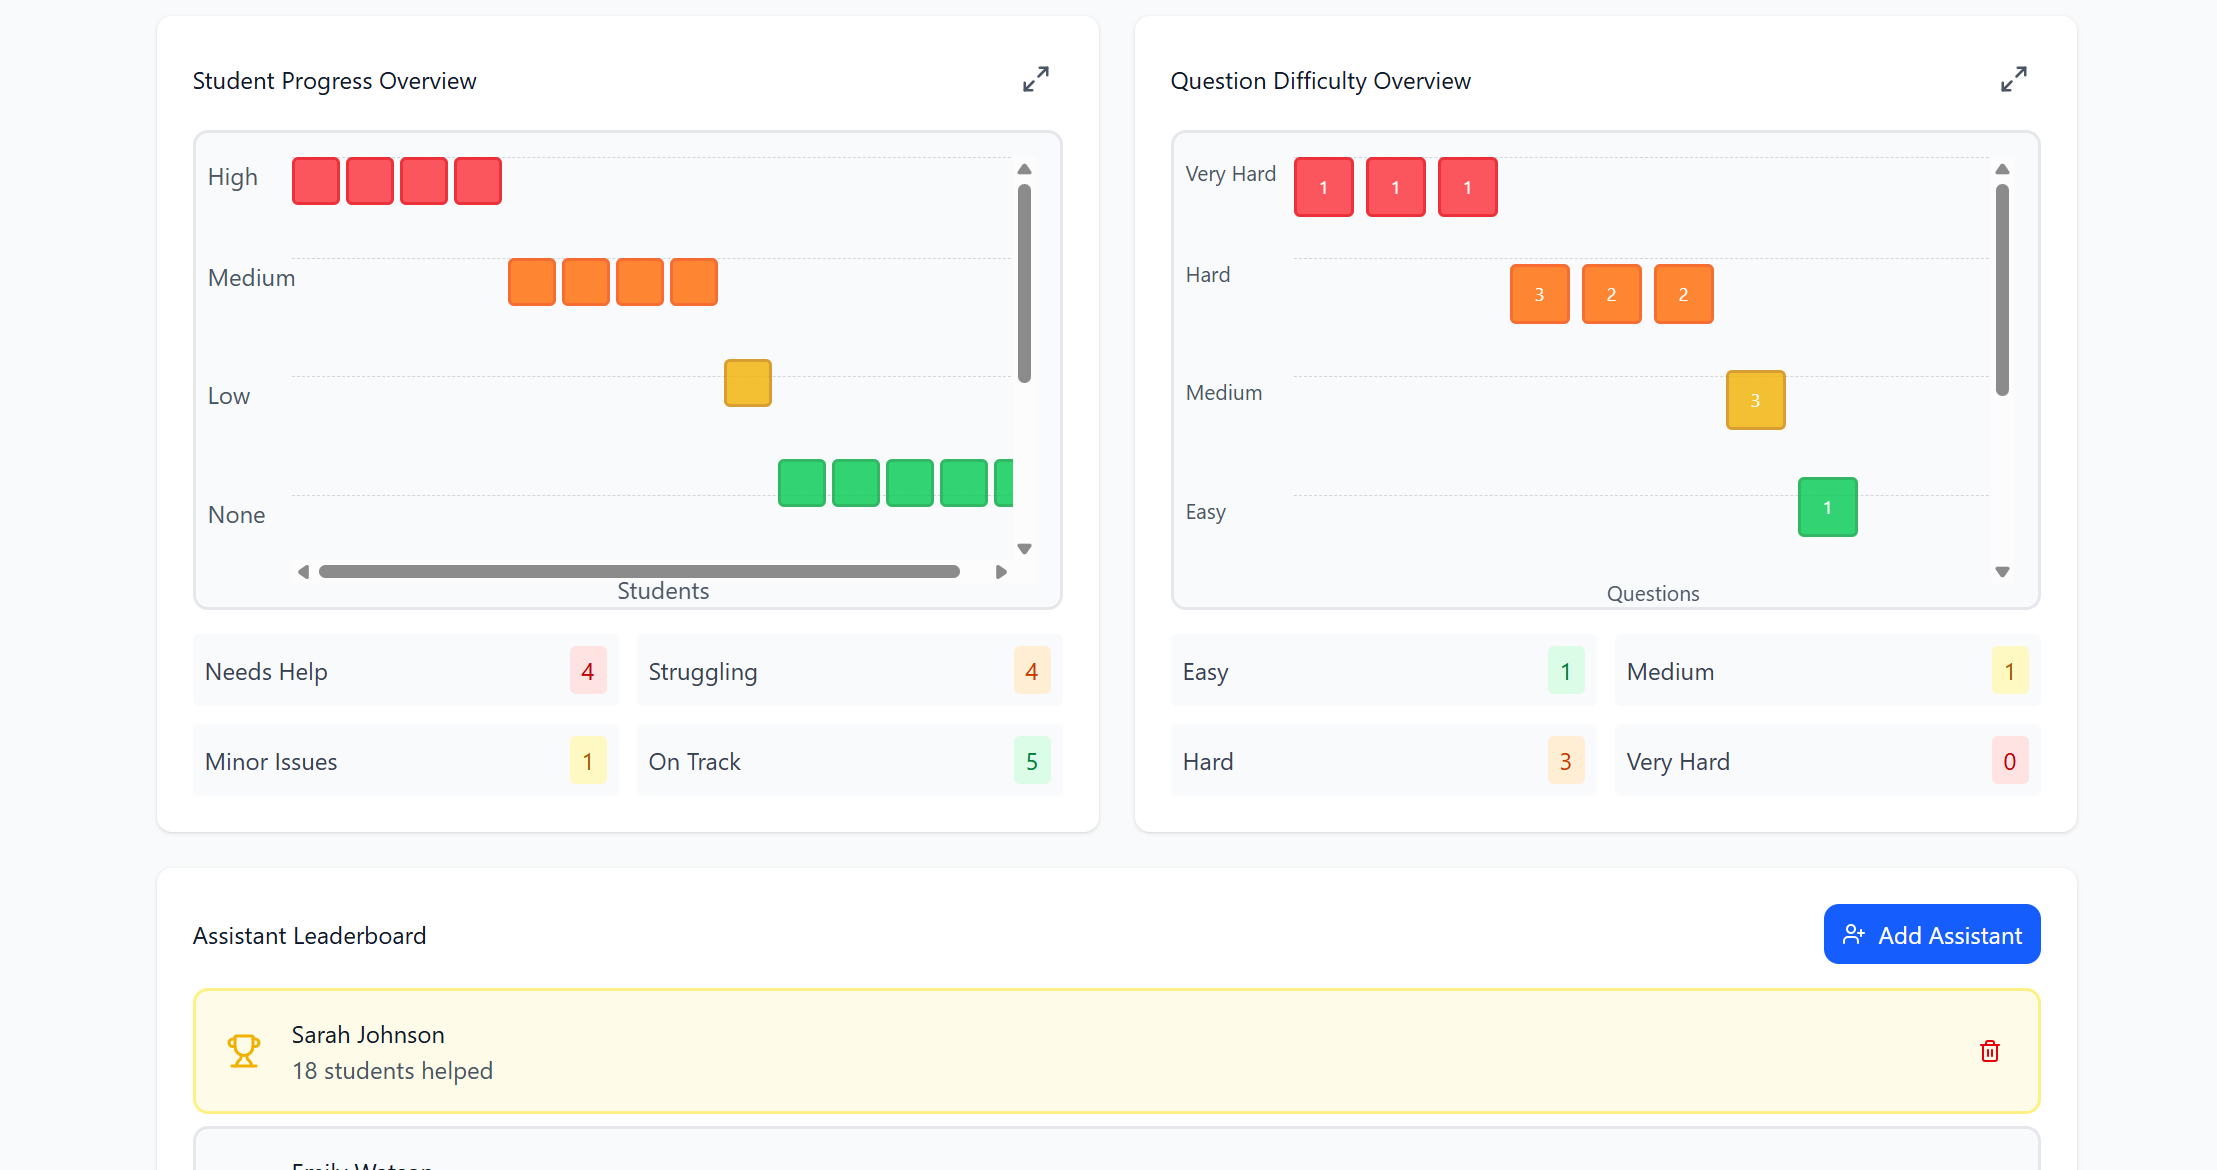
\includegraphics[width=1\linewidth]{figures/design-and-architecture/figma1.png}
    \caption{Views based on student struggle and question difficulty}
    \label{fig: figma1}
\end{figure}
As shown in Figure \ref{fig: figma1}, our dashboard has two key views: the first shows a list of students whose struggles are at certain thresholds, hence the colour; the second shows a list of questions based on difficulty at a threshold, thus the colour. The values used for comparison against the thresholds are derived from our student struggle and question difficulty equations. The view also allows instructors to go over additional information.

\begin{figure}[H]
    \centering
    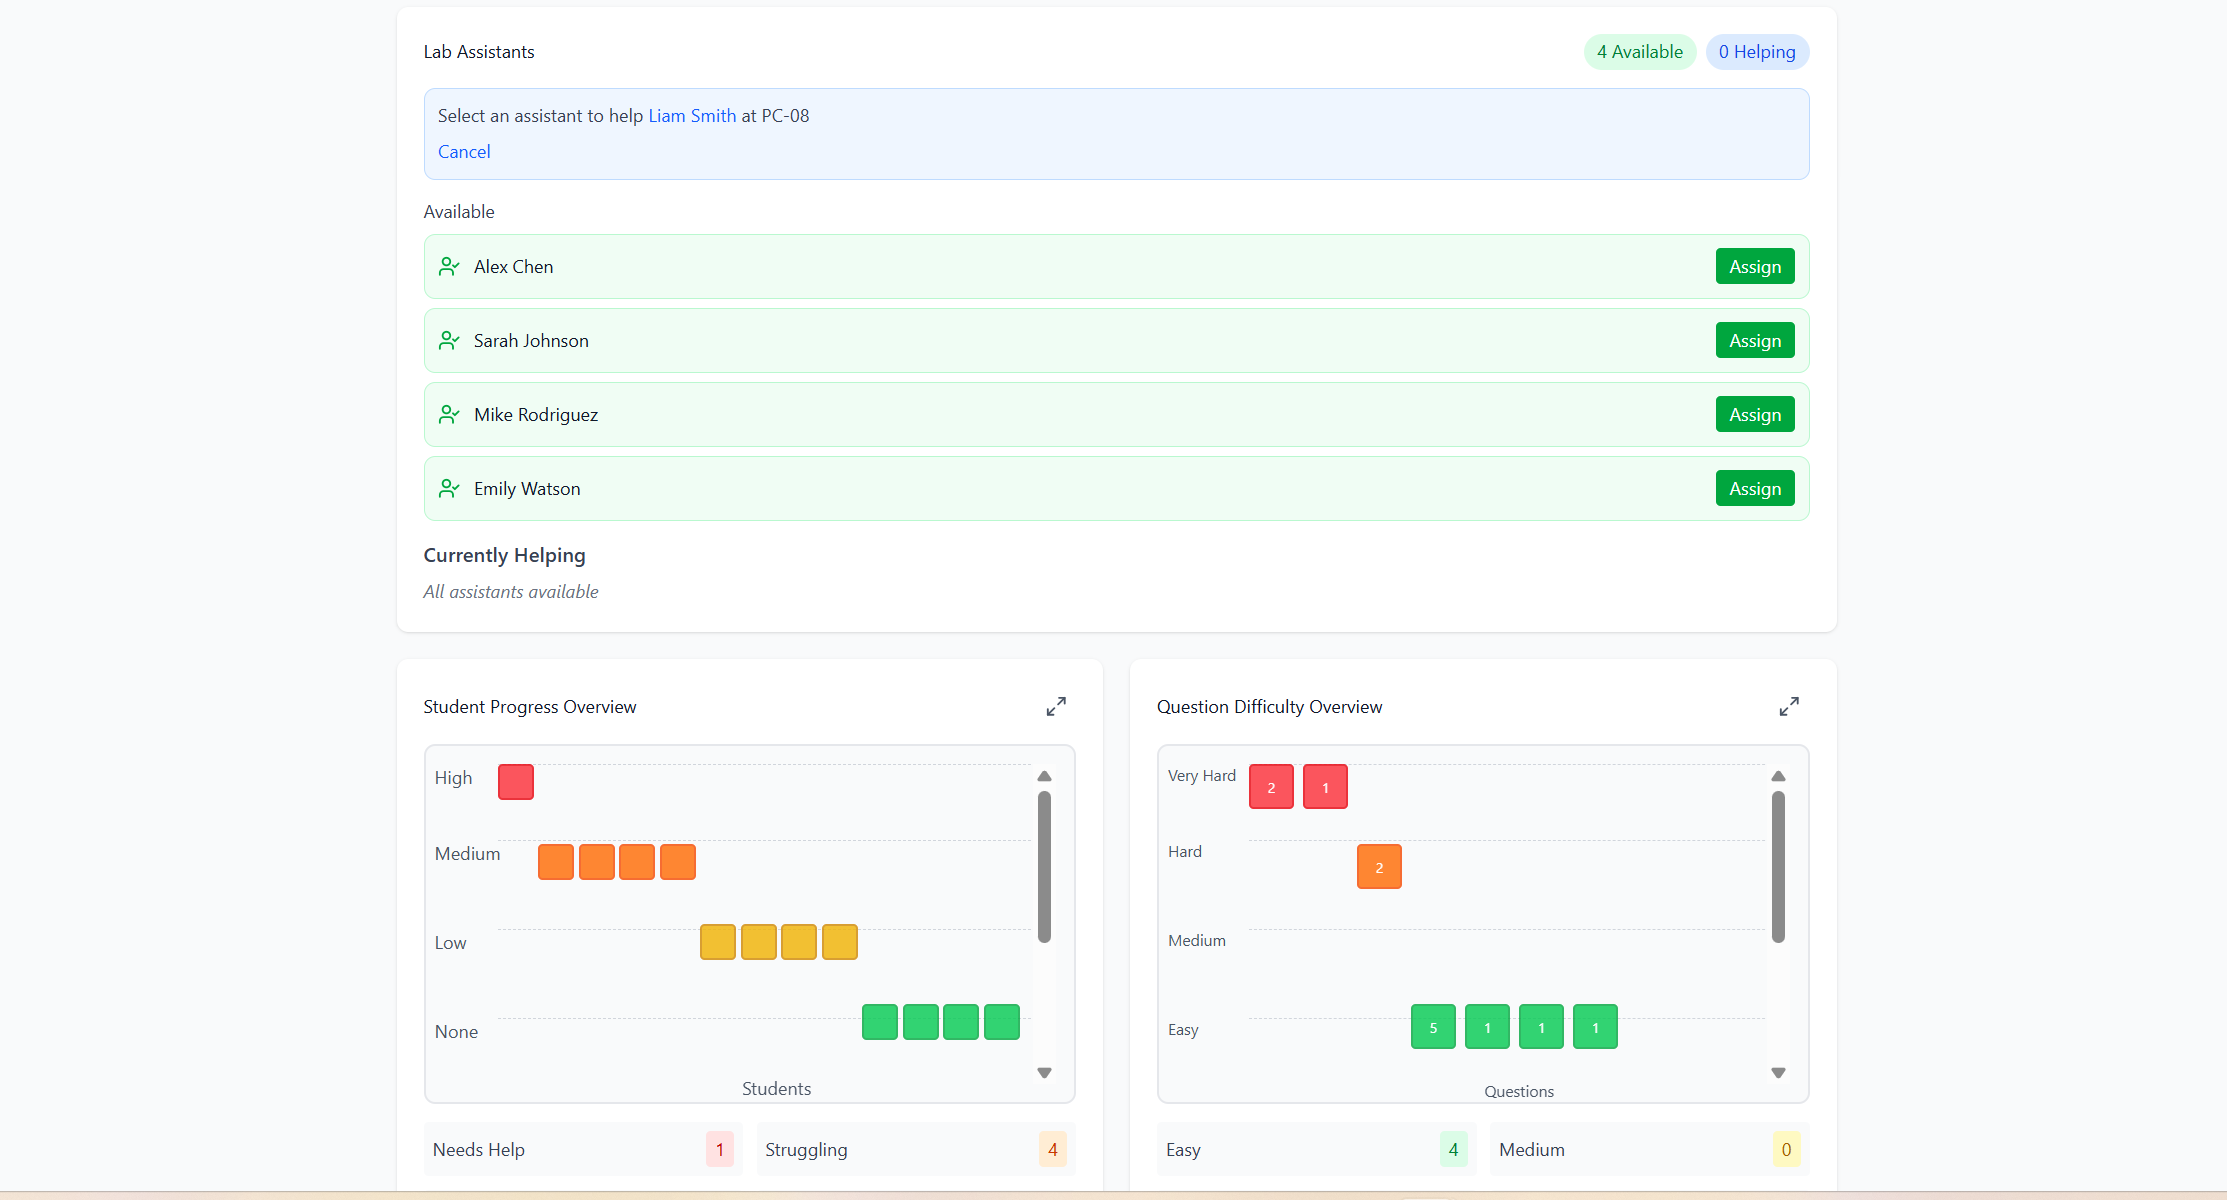
\includegraphics[width=1\linewidth]{figures/design-and-architecture/figma2.png}
    \caption{View of allocation of Lab Assistant}
    \label{fig: figma2}
\end{figure}
In Figure \ref{fig: figma2}, we can select a lab assistant and then press a student to allocate them. This is a simple approach and a very minimal, intuitive design that allows use without training on the system.


\begin{figure}[H]
    \centering
    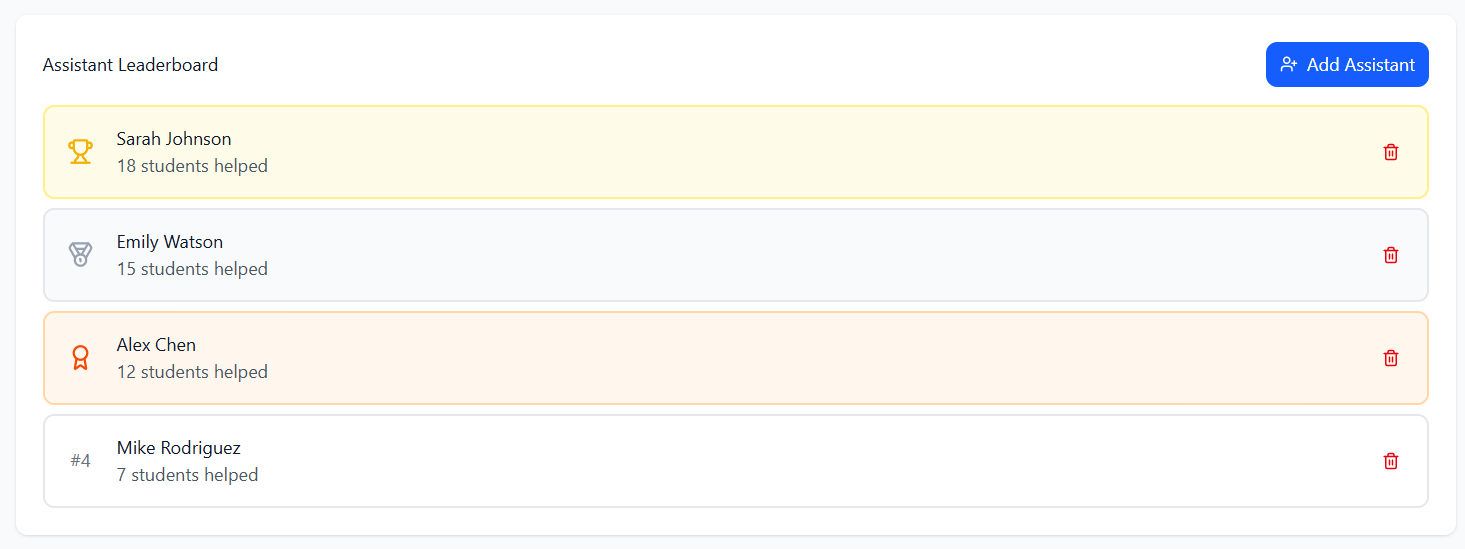
\includegraphics[width=1\linewidth]{figures/design-and-architecture/figma3.png}
    \caption{Assistant leaderboard, based on how many students have been helped}
    \label{fig: figma3}
\end{figure}
In Figure \ref{fig: figma3}, we can see that lab assistants are displayed based on their contributions. By gamifying the helping process, we can incentivise assistants to help more students.

\subsubsection{Lab Assistant View}

The lab assistant view is the mobile interface designed for assistants moving between students during a live session. Unlike the lab instructor dashboard, which assumes a stationary screen and wide canvas, the assistant view is built for short interactions on a handheld device. The interface presents one of three states at any moment, each scoped to the assistant's current responsibility: joining a session, waiting for an assignment, or helping the student they have been assigned. Figure~\ref{fig: assistant views} shows the three states in sequence.

\begin{figure}[H]
    \centering
    \begin{subfigure}[t]{0.31\linewidth}
        \centering
        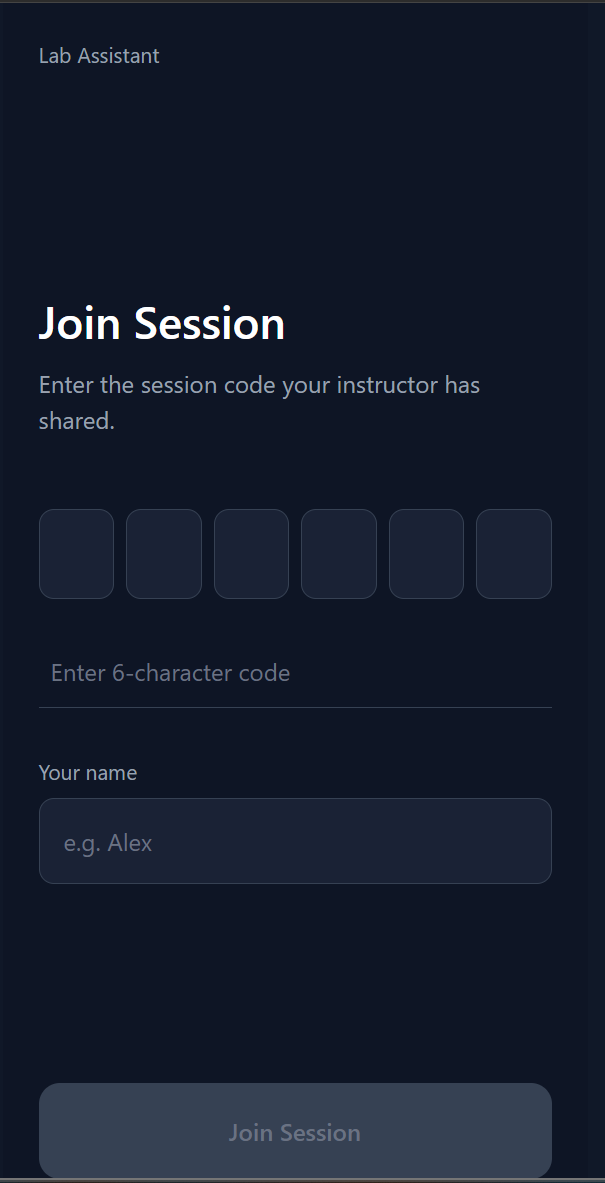
\includegraphics[width=\linewidth]{figures/design-and-architecture/figma4.png}
        \caption{Session join}
        \label{fig: figma4}
    \end{subfigure}
    \hfill
    \begin{subfigure}[t]{0.31\linewidth}
        \centering
        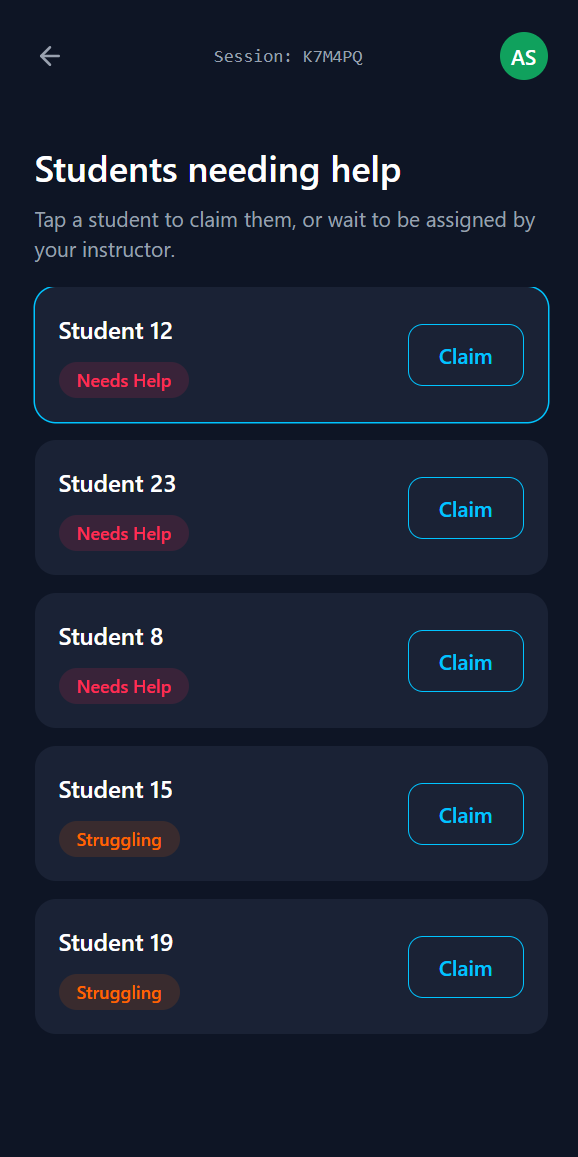
\includegraphics[width=\linewidth]{figures/design-and-architecture/figma5.png}
        \caption{Waiting for assignment}
        \label{fig: figma5}
    \end{subfigure}
    \hfill
    \begin{subfigure}[t]{0.31\linewidth}
        \centering
        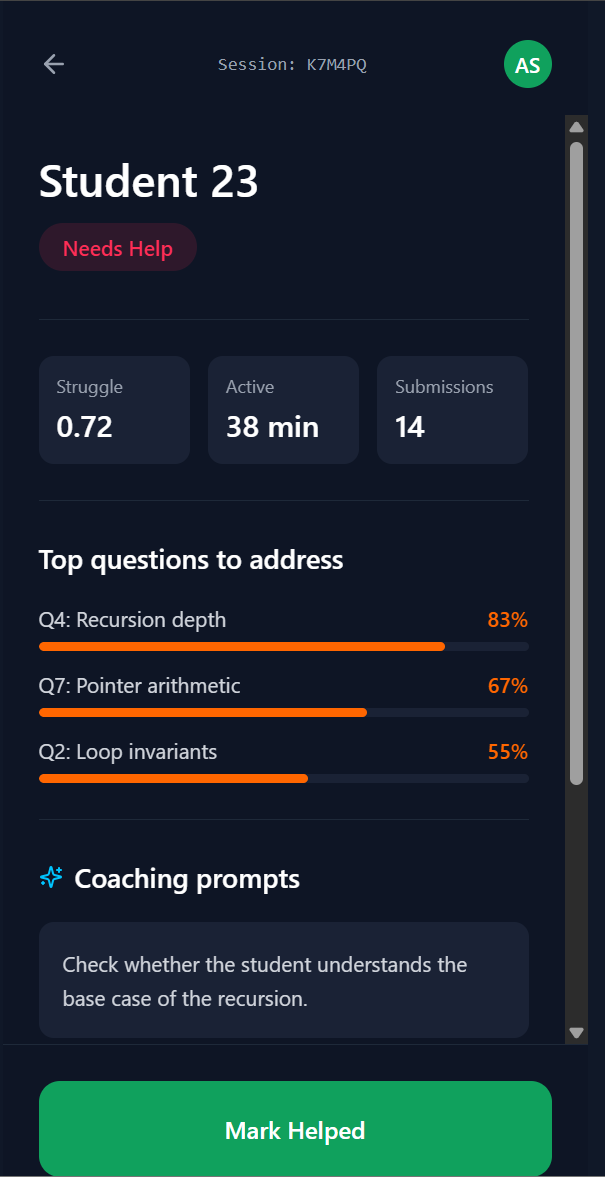
\includegraphics[width=\linewidth]{figures/design-and-architecture/figma6.png}
        \caption{Assigned student}
        \label{fig: figma6}
    \end{subfigure}
    \caption{The three states of the lab assistant view: \subref{fig: figma4} the session-join screen where the assistant enters the session code and their name; \subref{fig: figma5} the waiting state with a priority list of unassigned struggling students; \subref{fig: figma6} the assigned-student card showing struggle context, prioritised questions, and coaching prompts from the RAG layer.}
    \label{fig: assistant views}
\end{figure}

On first access (Figure~\ref{fig: figma4}), the assistant enters the session code shown on the instructor dashboard and provides their name. The session code is short enough to be read aloud by the instructor and typed without errors; the name is recorded so subsequent allocation decisions can address assistants individually. Once joined, the assistant is enrolled in the session and remains until they leave, are removed, or the session ends.

Between assignments (Figure~\ref{fig: figma5}), the assistant sees a ranked list of students currently flagged for help, ordered by their struggle score. The assistant may wait for the instructor to allocate them directly, or self-claim a student from the list when the instructor has enabled this. The same list is visible to every joined assistant; once a student is claimed, they are removed from the unassigned pool so two assistants cannot end up at the same desk.

Once a student is assigned (Figure~\ref{fig: figma6}), the view collapses to a single student card carrying the information the assistant needs at the desk: the student's current struggle context, the questions they are most incorrect on, and a short list of coaching prompts retrieved from the RAG layer described in Section~\ref{sec:rag}. A Mark Helped action lets the user know the student was helped, after which the assistant can either release the student or continue providing assistance.

\subsubsection{Visual Encoding of Metrics}

By deciding on thresholds, we can highlight a student by degree of struggle or highlight a question by degree of difficulty


\begin{table}[H]
    \centering
    \begin{tabular}{|p{0.1\textwidth}||p{0.2\textwidth}|p{0.2\textwidth}|p{0.2\textwidth}|p{0.2\textwidth}|}
    \hline
        Degree & \cellcolor{tlGreen}On Track & \cellcolor{tlAmber}Minor Issues & \cellcolor{tlOrange}Struggling & \cellcolor{tlRed}Needs Help \\
    \hline
        Threshold & $0 \leqslant S_t(s,\sigma) \leqslant t_{s1}$ & $t_{s1} < S_t(s,\sigma) \leqslant t_{s2}$&  $t_{s2} < S_t(s,\sigma) \leqslant t_{s3}$ &  $t_{s3} < S_t(s,\sigma) \leqslant 1 $\\
    \hline
    \end{tabular}
    \caption{Table Highlighting how thresholds can be indicated for struggle}
    \label{tab: struggle table}
\end{table}

\begin{table}[H]
    \centering
    \begin{tabular}{|p{0.1\textwidth}||p{0.2\textwidth}|p{0.2\textwidth}|p{0.2\textwidth}|p{0.2\textwidth}|}
    \hline
        Degree & \cellcolor{tlGreen}Easy & \cellcolor{tlAmber}Medium & \cellcolor{tlOrange}Hard & \cellcolor{tlRed}Very Hard\\
    \hline
        Threshold & $0 \leqslant D_t(q) \leqslant t_{s1}$ & $t_{s1} < D_t(q) \leqslant t_{s2}$&  $t_{s2} < D_t(q) \leqslant t_{s3}$ &  $t_{s3} < D_t(q) \leqslant 1 $\\
    \hline
    \end{tabular}
    \caption{Table Highlighting how thresholds can be indicated for difficulty}
    \label{tab: difficulty table}
\end{table}
